% =====================================================================
% Aspect Recoverability: a negative feasibility study
%
% CITATION STATUS
%   Six references below were verified during preparation and carry a
%   [VERIFIED] marker in the bibliography. Every other citation point is
%   marked \needcite{...} and MUST be filled from Scopus or Web of Science
%   before submission. Do not remove a \needcite marker without adding a
%   reference that has been checked to exist.
%
%   The \needcite command prints a visible red marker so no placeholder can
%   survive to submission unnoticed. Set \draftmode to false to make them
%   invisible only after all have been resolved.
% =====================================================================

\documentclass[11pt,a4paper]{article}

\usepackage[utf8]{inputenc}
\usepackage[T1]{fontenc}
% Times-compatible text and maths, the default expectation at most Elsevier,
% Springer and Wiley titles. Helvetica for sans elements, Courier for code.
\usepackage{mathptmx}
\usepackage[scaled=0.90]{helvet}
\usepackage{courier}
\usepackage{microtype}
\usepackage{siunitx}
\usepackage[hang,small,bf,labelsep=period]{caption}
\usepackage{lineno}
\usepackage{orcidlink}
\usepackage[margin=2.5cm]{geometry}
\usepackage{graphicx}
\usepackage{booktabs}
\usepackage{amsmath}
\usepackage{amssymb}
\usepackage{xcolor}
\usepackage{caption}
\usepackage{subcaption}
\usepackage{hyperref}
\usepackage{url}
\usepackage{natbib}
\usepackage{authblk}
\usepackage{placeins}
\usepackage{float}

% Keep floats near their callouts. Without this, ten figures in a 16-page
% article drift to the end and land inside the bibliography.
\renewcommand{\topfraction}{0.9}
\renewcommand{\bottomfraction}{0.8}
\renewcommand{\textfraction}{0.07}
\renewcommand{\floatpagefraction}{0.75}
\setcounter{topnumber}{3}
\setcounter{bottomnumber}{2}
\setcounter{totalnumber}{4}

% Flush all pending floats at every section boundary.
\makeatletter
\AtBeginDocument{%
  \let\original@section\section
  \renewcommand{\section}{\FloatBarrier\original@section}%
  \let\original@subsection\subsection
  \renewcommand{\subsection}{\FloatBarrier\original@subsection}%
}
\makeatother

\hypersetup{colorlinks=true, linkcolor=black, citecolor=black, urlcolor=blue,
  pdftitle={Aspect-Level Sentiment Decline and Return Is Not Estimable from Two Large Public Review Corpora},
  pdfauthor={S. Vakil and Y. Farjami}}

% Line numbers assist reviewers; remove for the camera-ready version.
\linenumbers
\renewcommand\linenumberfont{\normalfont\tiny\sffamily\color{gray}}

\captionsetup[table]{skip=4pt}
\captionsetup[figure]{skip=6pt}
\setlength{\tabcolsep}{5pt}
\renewcommand{\arraystretch}{1.12}
\sisetup{detect-weight=true, detect-family=true}

\newif\ifdraftmode
\draftmodefalse   % no placeholders remain; markers are off

\newcommand{\needcite}[1]{%
  \ifdraftmode\textcolor{red}{\textsuperscript{[CITE: #1]}}\fi}

\title{Aspect-Level Sentiment Decline and Return Is Not Estimable from Two
Large Public Review Corpora: A Negative Feasibility Study with a Density Bound}

\author[1]{S. Vakil\,\orcidlink{0009-0009-1336-5045}\thanks{Corresponding author.}}
\author[1]{Y. Farjami\,\orcidlink{0000-0003-1908-8826}}
\affil[1]{Department of Computer Engineering, Faculty of Engineering,
University of Qom, Qom, Iran}

\date{}

\begin{document}
\maketitle

\begin{abstract}
\noindent
Review-analytics work routinely models how sentiment toward a product attribute
evolves after a negative event and reads the return of sentiment as recovery.
We asked whether that construct is estimable at all from public review corpora.
Operational definitions of shock, recovery and censoring were fixed in a
version-controlled protocol before any data were inspected, then applied to
Amazon Reviews 2023 and MobileRec. At the product level, 313 of 11{,}925
product-months met a 30-mention threshold (2.6\,\%) and no shock was detected;
a denser extract yielded five analysable episodes against the 65 events needed
to detect a hazard ratio of 2.0 at 80\,\% power. Aggregating to category level
restored whole-review density (955 qualifying category-months) but not
identifiability at the aspect level, where the series do not form at all. At
category level, where whole-review series do exist, the picture is mixed and we
report it as such: a threshold rule found 23 shocks against $28.4 \pm 3.8$
expected under a circular block bootstrap null at 999 replicates, a ratio of
0.81 with empirical $p = 0.95$, while PELT applied to the same series found six
change points against $1.77 \pm 1.35$ expected, a ratio of 3.40 at $p = 0.015$
uncorrected, or $p = 0.060$ under Bonferroni across the four tests performed. A
positive control shows why the first result is weak evidence of anything: the
threshold criterion fires on every clean synthetic series and recovers only
two-thirds of injected two-standard-deviation shocks. We therefore claim
neither presence nor absence of structure at category level, since our
criterion cannot distinguish them; the claim we do make is narrower, that the
aspect-level series required to study the question do not exist. An unvalidated lexicon measure, reported for
robustness only, likewise fails to reject, though it differs from the star
rating on outcome composition and censoring and should not be described as
agreeing with it. Returning to the aspect level, none of 7{,}084 aspect cells reached
the threshold, at a median of one mention per cell. We derive a density bound: the number of aspects that can reach the threshold
is at most $Rm/T$, for $R$ reviews per unit-period, $m$ aspects named per review
and threshold $T$. At $T = 30$ the bound caps MobileRec at $1.16m$ aspects and
Amazon at $0.23m$. We did not measure $m$, so the cap is conditional on it, and
we report the bound's sensitivity to both $m$ and $T$ rather than asserting a
single number. Repeat
reviewing of the same item runs at 0.159\,\% and 0.063\,\% in the two corpora,
so recovery of an average cannot be separated from turnover in who is
reviewing. The obstacle is the quantity of text, not the choice of method.
\end{abstract}

\vspace{4pt}
\noindent\fbox{\parbox{0.97\textwidth}{\small
\textbf{Data and code.} Every figure, table and number in this article is
reproduced by the scripts and protocol archived at\\
\url{https://github.com/ssvakil/aspect-recoverability}\\
The archive contains the operational definitions fixed before data inspection,
the analysis code with its self-test suite, and the figure generation script.}}

\vspace{6pt}
\noindent\textbf{Keywords:} online reviews; sentiment dynamics; negative
results; survival analysis; construct validity; reproducibility

\section{Introduction}

Online reviews are routinely mined for signals about how customer perception
changes over time. Aspect extraction from review text dates to \citet{hu2004} and remains
active \citep{zhou2023}. A recurring pattern in the applied literature is to
construct an attribute-level sentiment series, identify a decline, observe
whether sentiment later returns, and interpret the return as recovery
\citep{park2024, roelen2023, yang2023}. The
managerial appeal is obvious: if some attributes recover and others do not,
firms could prioritise repairs accordingly.

Our study began as an attempt to formalise this idea as a time-to-event
problem. We intended to model the time from an attribute-level sentiment shock to
recovery, treating episodes that had not recovered by the end of the horizon as
administratively censored rather than as a distinct event type, and to test
whether non-recovering shocks predicted subsequent customer disengagement. Before
committing to that analysis we did what is rarely reported: we asked whether
the data could support it.

It cannot. This paper reports why, and we argue the reasons generalise beyond
our particular design.

Our contribution is threefold. First, we provide a quantified feasibility
assessment of attribute-level recovery estimation on two corpora that are
standard in this literature, showing that the required longitudinal density is
absent by one to two orders of magnitude. Second, we identify a construct
validity problem that applies to any population-level recovery claim: because
repeat reviewing is rare, recovery of an average is not separable from
turnover in who is averaged. Third, we show that the choice of null control
matters materially, and that the permutation null most readily available is
biased toward declaring detection successful.

Negative feasibility results are underreported, which means the same
infeasible designs are attempted repeatedly. Publication bias toward positive
findings is long documented \citep{rosenthal1979, easterbrook1991, fanelli2010}, operates through non-writeup as well as non-acceptance
\citep{franco2014}, and motivates registered reports \citep{chambers2013} and
broader open-research norms \citep{nosek2015, ioannidis2005}. Feasibility
failures are a costly omission in particular, because the cost of
rediscovering them falls on every group that attempts the design. We therefore report our thresholds, our pre-specified definitions, and our
failure points in full.

\section{Related work}

\subsection{Attribute-level sentiment over time}

That customer evaluations of specific attributes shift over the consumption
cycle is long established. \citet{mittal1999} analysed longitudinal data from
5{,}206 automobile owners and showed that attribute-level performance,
satisfaction, and behavioural intentions must be examined intertemporally
because the relationships among them change as consumption proceeds, with
attribute weights shifting according to their salience over time. Later
computational work reaches compatible conclusions with different
methods \citep{park2024, roelen2023}. Adjacent work in requirements
engineering classifies app reviews into actionable categories
\citep{maalej2015}, the closest analogue to attribute extraction in the mobile
setting.

\citet{xia2021} model the dynamic evolution of user preferences and item
features at the aspect level, detecting both gradual drift and abrupt change
points across three real-world datasets. Their work establishes that
aspect-level series contain detectable structure; our results are not in
conflict with theirs, since we address a narrower question about a specific
event-based construct.

\subsection{Recovery after failure}

The marketing literature has examined recovery for decades. The service
recovery paradox holds that a well-handled failure can leave a customer more
satisfied than if nothing had gone wrong. The meta-analysis by
\citet{dematos2007} found support for this only in post-recovery satisfaction,
with an effect size of 0.125, and no significant effect on repurchase
intentions --- that is, recovered satisfaction does not ensure loyalty. They
further report that study design, subject type, and service category moderate
the effect, and characterise the underlying body of findings as inconsistent.

Two features of that literature are relevant here. It measures stated
constructs in scenario settings rather than observed behaviour, and its unit
of analysis is a failure episode involving a firm response. Our design
observes behaviour but cannot observe the firm response, which is why we
framed the construct as perceptual rather than managerial.

Negativity bias is a standing explanation for why declines and recoveries need
not be symmetric \citep{baumeister2001, rozin2001}: negative information is
weighted more heavily and is more resistant to disconfirmation than positive
information of comparable magnitude. Asymmetry between satisfaction and
switching is also long documented:
\citet{labarbera1983} found that repurchase of a brand was influenced by
lagged intention, whereas switching behaviour was more sensitive to
dissatisfaction with brand consumption.

\subsection{How this study differs}
\label{sec:comparison}

Table~\ref{tab:related} positions the present study against the work closest to
it on the dimensions that decide whether recovery is estimable. The columns are
not measures of quality: the studies listed answer questions of their own, and
most had no reason to report what we look for here. They are the properties a
recovery analysis needs.

Three patterns emerge. Work that observes real behaviour at the attribute level
is cross-sectional or models gradual drift, not discrete events. Work that
treats failure and recovery as events comes from service marketing and measures
stated intention in scenario settings rather than observed behaviour. And no
study in either group reports whether its data were dense enough to support the
analysis attempted, which is the question this paper is about.

\begin{table}[htbp]
\centering
\caption{The present study against the closest prior work. \textbf{Obs.}:
observational data rather than survey or scenario. \textbf{Long.}: repeated
measurement over time. \textbf{Event}: failure and recovery treated as discrete
events rather than as gradual drift. \textbf{TTE}: a time-to-event model.
\textbf{Null}: a resampling null against which detections are compared.
\textbf{Density}: feasibility of the data for the analysis attempted is
reported. Characterisations follow each study's published account of its own
design.}
\label{tab:related}
\small
\begin{tabular}{@{}llcccccc@{}}
\toprule
\textbf{Study} & \textbf{Unit} & \textbf{Obs.} & \textbf{Long.} &
\textbf{Event} & \textbf{TTE} & \textbf{Null} & \textbf{Density} \\
\midrule
\multicolumn{8}{@{}l}{\textit{Attribute extraction and ranking from reviews}} \\
\citet{hu2004}          & aspect    & yes & no  & no  & no & no & no \\
\citet{maalej2015}      & review    & yes & no  & no  & no & no & no \\
\citet{zhou2023}        & feature   & yes & no  & no  & no & no & no \\
\citet{roelen2023}      & attribute & yes & no  & no  & no & no & no \\
\citet{yang2023}        & attribute & yes & no  & no  & no & no & no \\
\citet{park2024}        & feature   & yes & no  & no  & no & no & no \\
\addlinespace
\multicolumn{8}{@{}l}{\textit{Temporal dynamics of attribute sentiment}} \\
\citet{xia2021}         & user\,$\times$\,item\,$\times$\,aspect
                                    & yes & yes & no  & no & no & no \\
\citet{mittal1999}      & attribute & no  & yes & no  & no & no & n/a \\
\addlinespace
\multicolumn{8}{@{}l}{\textit{Failure and recovery}} \\
\citet{labarbera1983}   & overall   & no  & yes & no  & no & no & n/a \\
\citet{dematos2007}     & episode   & no  & mix & yes & no & no & n/a \\
\addlinespace
\multicolumn{8}{@{}l}{\textit{This study}} \\
Present work            & aspect\,$\times$\,unit\,$\times$\,month
                                    & yes & yes & yes & attempted & yes & yes \\
\bottomrule
\end{tabular}
\end{table}

The final row reads "attempted" rather than "yes" deliberately. We specified a
time-to-event analysis and could not run it, and the reason is the subject of
this paper. Marking it "yes" would claim a contribution we did not make.

The comparison also shows why the gap persisted. A study needs observational
data for behaviour, longitudinal structure for dynamics, and an event framing
for recovery. The first two are common; the third belongs to a literature that
works with surveys and scenarios. Combining all three is what exposes the
density constraint, and it is only visible once the combination is attempted.

\subsection{What has not been done}
\label{sec:gap}

We found no prior work that models attribute-level recovery as a time-to-event
outcome on naturally occurring longitudinal review data, or that separates
recovery of the original reviewer cohort from recovery of the population
average. We state this carefully: our search was targeted rather than
systematic, so it establishes that we did not find such work, not that none
exists (Section~\ref{sec:limitations}). That apparent absence motivated the
study. Our results suggest one reason for it.

\section{Method}

\subsection{What the construct is, and is not}
\label{sec:construct}

A clarification that bears on every result below. We observe no intervention
dates, no product releases, no recalls and no firm responses. A "shock" here is
a sustained fall in measured sentiment, identified from the series itself, and
"recovery" is a return of that series toward its earlier level.

This is therefore a study of \emph{sentiment decline and return}, not of
service recovery in the sense of \citet{dematos2007}, where a failure event and
a firm response are both observed and the outcome is satisfaction or stated
intention. The two constructs share a shape and little else. Where we use the
word recovery we mean the former, and no claim about the latter follows from
our results.

The distinction also limits the interpretation available even had detection
succeeded. A series that falls and returns is consistent with a defect
introduced and repaired, with a change in who is reviewing, with a seasonal
effect, and with a shift in platform ranking. Without intervention dates these
are not separable, which is why Section~\ref{sec:whatdata} lists documented
intervention timestamps among the data properties a usable study would need.

\subsection{Pre-specified definitions}

All definitions in Table~\ref{tab:definitions} were fixed before any data were
inspected and are archived in the repository. No threshold or classification
rule was changed after data inspection. One deviation of scope was made and is
recorded in the deviation log: after the product- and app-level analyses proved
infeasible, the unit of analysis was moved to the app category. That analysis
was not covered by the protocol and is reported as exploratory throughout.

Table~\ref{tab:definitions} also lists the disengagement definition, which
belonged to the planned downstream analysis. That analysis was never reached,
and no disengagement result is reported here.

\begin{table}[htbp]
\centering
\caption{Operational definitions, fixed before data inspection.}
\label{tab:definitions}
\small
\begin{tabular}{@{}p{3.4cm}p{10.2cm}@{}}
\toprule
\textbf{Construct} & \textbf{Definition} \\
\midrule
Qualifying month & At least 30 mentions in that unit-month; months below the
threshold are dropped and never interpolated \\
Baseline & Mean sentiment over the six months preceding shock onset \\
Negative shock & Drop of at least $1$ SD below baseline, sustained for at
least two consecutive months \\
Recovery & Return to at least 90\,\% of baseline, sustained for at least three
consecutive months \\
Non-recovery & No recovery within 18 months, \emph{with the full 18 months
observed} \\
Right-censored & Fewer than 18 months of post-shock data available \\
Disengagement & No further review of the brand for 12 months, conditional on
the user reviewing elsewhere in that window \\
\bottomrule
\end{tabular}
\end{table}

The censoring rule deserves emphasis. A shock occurring late in the
observation window can never be observed to recover. Classifying such episodes
as non-recovered rather than censored inflates estimated irreversibility
systematically, and the size of the inflation grows with the recovery horizon.

\subsection{Detection procedure}

Monthly sentiment series were constructed per unit, filtered to qualifying
months, and split at gaps so that no shock could be detected across a
discontinuity. Shocks were located by comparison against a trailing baseline window, then
classified as recovered, non-recovered, or censored according to
Table~\ref{tab:definitions}. The protocol named the PELT algorithm \citep{killick2012}, available as
described by \citet{killick2014}, as a robustness check on shock localisation,
with Bayesian online change point detection \citep{adams2007} as a sequential
alternative and the formulations of \citet{barry1993} and \citet{fearnhead2007}
as further options. None of these was run. The feasibility constraints reported
in Section~\ref{sec:results} removed the need: a robustness check on the
location of shocks is only meaningful once shocks are distinguishable from
noise, which they were not. All reported counts therefore use the threshold
rule, which is transparent and tied directly to the pre-specified
definitions.

\subsection{Null controls}
\label{sec:nulls}

Detection procedures of this kind will find events in pure noise, so an
explicit null is required. We report two.

The obvious null is a permutation of the series. This is biased. Real
sentiment series are autocorrelated, so adjacent months resemble one another
and the local standard deviation of a trailing window is small. Permutation
destroys that autocorrelation and inflates the local standard deviation, which
raises the detection threshold and mechanically suppresses shock counts. A
comparison against a permutation null therefore favours the hypothesis being
tested.

We instead use a circular block bootstrap \citep{politis1992}, a variant of the
moving block bootstrap \citep{kunsch1989} that wraps the series on a circle to
remove edge effects, and which preserves short-range autocorrelation while
randomising where episodes fall in time. The stationary bootstrap
\citep{politis1994} would serve equally; we fix the block length rather than
drawing it geometrically, and note that automatic block-length selection
\citep{politis2004, patton2009} would be preferable in a confirmatory study. Our
implementation includes a self-test demonstrating, on a synthetic AR(1) series
containing no injected shocks, that the permutation null returns fewer shocks
than the block bootstrap null.

Blocks are of fixed length six months, set equal to the baseline window so that
within-baseline dependence is preserved inside a single block; the length was
not tuned. We draw 999 replicates, giving a Monte Carlo standard error of the
null mean of $3.77/\sqrt{999} = 0.12$ shocks against a null standard deviation
of 3.77. All $p$-values are empirical quantiles of the bootstrap distribution
under the $(b+1)/(B+1)$ convention, which prevents a $p$ of exactly zero. Block
length was varied over 3, 6 and 12 months as a check: the observed-to-null
ratio moves only from 0.78 to 0.85 under star ratings, so the conclusion does
not rest on the value chosen.

\subsection{Power}

The planned analysis was a Cox proportional hazards model \citep{cox1972},
preceded by Kaplan--Meier estimation of time to recovery \citep{kaplan1958}.
Schoenfeld's formula \citep{schoenfeld1983} gives the number of \emph{events},
not observations, required to detect a hazard ratio:
\begin{equation}
d = \frac{(z_{1-\alpha/2} + z_{1-\beta})^{2}}{p(1-p)\,(\ln \mathrm{HR})^{2}},
\end{equation}
where $p$ is the exposed fraction. At $\alpha = 0.05$, 80\,\% power, and
balanced exposure, detecting $\mathrm{HR} = 2.0$ requires 65 events and
$\mathrm{HR} = 1.5$ requires 191. Because censored episodes contribute
person-time but not events, the number of episodes needed exceeds these
figures.

We also report events per parameter (EPP), since Schoenfeld's formula assumes a
single covariate of interest and the planned model has more. The conventional
floor of ten events per parameter derives from \citet{peduzzi1996}; it has been
argued relaxable in some circumstances \citep{vittinghoff2007} and challenged
as lacking a general rationale \citep{vansmeden2016}. We report EPP at three
and six parameters so the reader may apply whichever standard they prefer.

\subsection{Immortal time in the recovery covariate}

Recovery status is determined over an 18-month window, which makes it a
time-dependent quantity. Entering it into a Cox model as a baseline covariate
would introduce immortal time bias: an episode cannot be labelled recovered
unless it survived long enough for recovery to be observed, so the recovered
group would contain disproportionately late-failing observations by
construction, and the model would report a protective effect of recovery that
is an artefact of the definition. The bias was first identified in cohort
studies of transplantation survival and has since been documented across many
pharmacoepidemiological studies \citep{suissa2007, suissa2008, levesque2010};
its structure and remedies are reviewed by \citet{platt2019} and
\citet{yadav2021}. We therefore specified recovery as a time-varying covariate,
with person-time accruing in the non-recovered state from shock onset and
switching at the month recovery is confirmed. Landmark analysis
\citep{mi2016} and the alternatives compared by \citet{karim2016} would be
acceptable substitutes; the time-varying specification was fixed in the protocol.

\subsection{Reproducibility}

The analysis code contains 77 self-tests covering shock classification, censoring
classification, power arithmetic, series segmentation, null construction, and
recovery attribution. Tests assert behaviour on series whose correct classification is known by
construction; for instance, that a truncated permanent decline is labelled
censored rather than non-recovered. These establish that the classification
logic is correct given a detection. They do not establish that detection
occurs, which is a separate property and is measured by the positive control of
Section~\ref{sec:poscontrol}. A further 78 cover the data loaders and the
figure generation script, giving 155 in total. All code, definitions, and test
suites are at \url{https://github.com/ssvakil/aspect-recoverability}.

\section{Data}

\subsection{Scope of the empirical claims}

We analysed a 500{,}000-interaction scan of MobileRec, about 2.6\,\% of its
19.3 million interactions, and an 82{,}041-review extract covering the 200
densest products of one Amazon category. Neither is the full corpus, and the
Amazon extract is deliberately non-representative: it selects dense products
because density is the resource the analysis consumes.

Our empirical statements are therefore about these subsamples at these
thresholds, and we have tried to phrase them that way throughout. The density
bound is the exception: it is arithmetic on $R$, $m$ and $T$, and applies to
whatever panel a study actually assembles. A larger scan would raise the
absolute counts but would not raise $R$, since $R$ is a rate; only reviewing
behaviour or a different sampling design would do that.

\subsection{Amazon Reviews 2023}

We used the public research release covering 571.54 million reviews from May
1996 to September 2023 \citep{hou2026}. Random
sampling is inappropriate here: the analysis consumes longitudinal density,
and a random sample of reviews spreads thinly across millions of products so
that no product reaches the mention threshold. We therefore selected the
densest products and retained all of their reviews. This trades
representativeness for density, and findings accordingly generalise to
heavily-reviewed products only.

\subsection{MobileRec}

MobileRec contains 19.3 million interactions across 10{,}173 apps from
0.7 million users, ordered chronologically and filtered to a 5-core \citep{maqbool2023}. The 5-core criterion means
each user reviewed five \emph{distinct} apps. This is not the same as
reviewing one app repeatedly, and only the latter supports cohort-level
recovery analysis --- a distinction that is easy to miss and that proved
decisive.

\section{Results}
\label{sec:results}

\subsection{Density is insufficient at the product level}

Table~\ref{tab:density} summarises the feasibility of each configuration
attempted. In Amazon Reviews 2023, the 200 densest products of a category
yielded 82{,}041 reviews spanning 2005--2023, of which 313 of 11{,}925
product-months (2.6\,\%) met the 30-mention threshold. Zero shocks were
detected. Repeating the analysis on the full extract rather than a subsample
produced the same result, confirming that this was not an artefact of
sampling.

\begin{table}[htbp]
\centering
\caption{Feasibility across configurations. Qualifying unit-months are those
meeting the 30-mention threshold. Scan size and observation period are stated
for every row because they differ, and shares computed on different
denominators are not directly comparable. Rows within a block share a basis.
Balanced-panel denominators were absent from an earlier version of this table
and have since been logged by re-running the analysis; they are the
category-months actually present in each panel, which falls below the product
of categories and months because sparse months are dropped.}
\label{tab:density}
\small
\begin{tabular}{@{}llrrrr@{}}
\toprule
\textbf{Configuration} & \textbf{Scan} & \textbf{Units} &
\textbf{Unit-months} & \textbf{Qualifying} & \textbf{Share} \\
\midrule
\multicolumn{6}{@{}l}{\textit{Full observation period}} \\
Amazon, product (All\_Beauty) & 82{,}041 & 200 & 11{,}925 & 313 & 2.6\,\% \\
MobileRec, app & 300{,}000 & n.r. & 128{,}251 & 271 & 0.2\,\% \\
MobileRec, app & 500{,}000 & 8{,}603 & 170{,}846 & 827 & 0.5\,\% \\
MobileRec, category & 500{,}000 & 48 & 5{,}134 & 2{,}286 & 44.5\,\% \\
\addlinespace
\multicolumn{6}{@{}l}{\textit{Window 2018-01 to 2021-12}} \\
MobileRec, category, unbalanced & 500{,}000 & 48 & 2{,}299 & 1{,}788 & 77.8\,\% \\
\quad presence $\geq$ 50\,\% & 500{,}000 & 48 & 2{,}291 & 1{,}589 & 69.4\,\% \\
\quad presence $\geq$ 75\,\% & 500{,}000 & 46 & 2{,}150 & 955 & 44.4\,\% \\
\quad presence $\geq$ 90\,\% & 500{,}000 & 10 & 453 & 0 & 0.0\,\% \\
\bottomrule
\end{tabular}
\end{table}

Figure~\ref{fig:cascade} shows the progression across the three full-period
configurations, which share a basis and are therefore comparable. MobileRec at
the app level is sparser than Amazon at the product level, at 0.5\,\% of
app-months qualifying against 2.6\,\%; a smaller 300{,}000-interaction scan of
the same corpus gives 0.2\,\%. Neither is close to usable.

\begin{figure}[htbp]
\centering
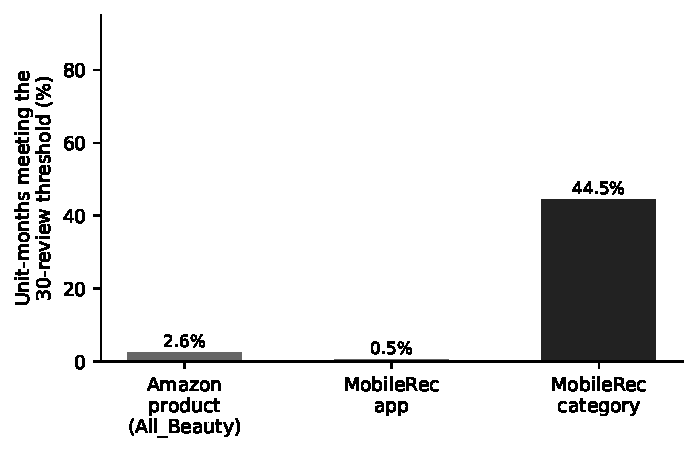
\includegraphics[width=0.72\textwidth]{figures/fig1_density_cascade.pdf}
\caption{Share of unit-months meeting the 30-mention threshold at each level of
aggregation, all over the full observation period on a 500{,}000-interaction
scan for MobileRec. The category figure here, 44.5\,\% (2{,}286 of 5{,}134),
is \emph{not} the 44.4\,\% quoted elsewhere: that is the windowed balanced
panel, 955 qualifying category-months out of a denominator the run did not
log. It lies below the $46 \times 48 = 2{,}208$ maximum, since sparse months
are dropped, but we do not state it, because recovering it by dividing 955 by
the reported share would be a derived figure presented as a measured one. The
two percentages are near-identical by coincidence and rest on different bases;
we flag this because the resemblance misled us during analysis.}
\label{fig:cascade}
\end{figure}

\subsection{Statistical power is unattainable at the product level}

% AUTHOR ACTION: name the category here from the run log before submission.
% A reviewer will ask which category this was; "a denser category" is not
% sufficient. Do not guess -- take it from the terminal output of the run.
A second Amazon extract, from a category with heavier reviewing than
All\_Beauty, produced five analysable episodes. Against the 65 events required for $\mathrm{HR} = 2.0$, this is
short by a factor of thirteen; against the 191 required for
$\mathrm{HR} = 1.5$, by a factor of thirty-eight.
Figure~\ref{fig:power} places all three configurations against both
requirements.

\begin{figure}[htbp]
\centering
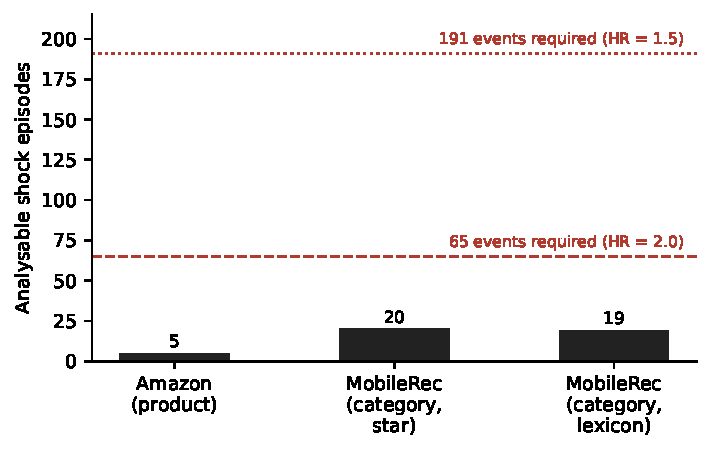
\includegraphics[width=0.72\textwidth]{figures/fig7_power_gap.pdf}
\caption{Analysable shock episodes obtained, against the events required by
Schoenfeld's formula at 80\,\% power: five for Amazon at product level, 20 for
the category panel under star ratings and 19 under lexicon polarity. No
configuration approaches either threshold.}
\label{fig:power}
\end{figure}

Inverting Schoenfeld's formula gives the smallest effect the obtained event
count could detect. With the 20 analysable episodes from the star-rating
measure, the minimum detectable hazard ratio at 80\,\% power is 3.50
(Figure~\ref{fig:powercurve}). Hazard ratios of that magnitude are not
plausible for the effect under study, so the design is not merely
underpowered but incapable of addressing the question at this sample size.

\begin{figure}[htbp]
\centering
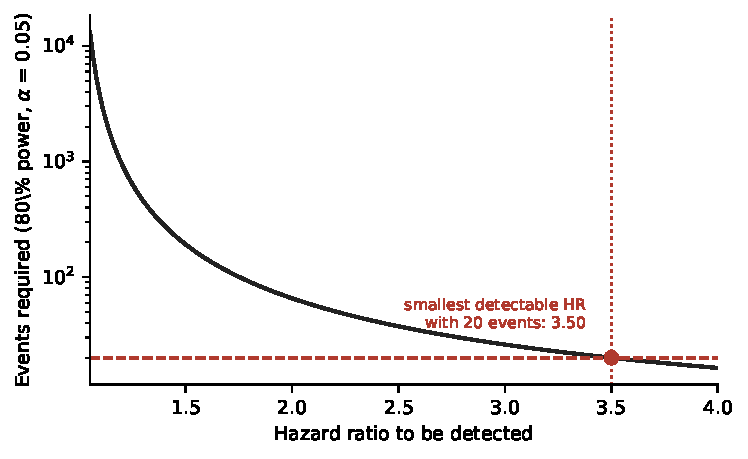
\includegraphics[width=0.68\textwidth]{figures/fig9_power_curve.pdf}
\caption{Events required as a function of the hazard ratio to be detected,
with the largest obtained episode count marked. The intersection gives the
minimum detectable effect.}
\label{fig:powercurve}
\end{figure}

\subsection{Cohort recovery is not computable}

In a 300{,}000-interaction sample of MobileRec, 188 of 299{,}812 user--app
pairs contained more than one review, a repeat rate of 0.063\,\%; within the
balanced panel it was 0.059\,\%. In the Amazon extract, 130 of 81{,}902
user--product pairs repeated, a rate of 0.159\,\%. Amazon reviewers return to
the same item about two and a half times as often as MobileRec users
(Figure~\ref{fig:repeat}).

Neither figure supports a cohort analysis, and the shortfall is not marginal.
With 23 shock episodes and a 0.159\,\% repeat rate, the expected number of
pre-shock reviewers who return after their shock is below one. We set a working
convention of 2\,\% in our code as the point below which the cohort estimate is
withheld rather than reported; that convention is ours and we know of no
standard for it, but the observed rates are more than an order of magnitude
below any threshold one might reasonably choose, so nothing in our conclusion
turns on where it is set. Measuring both matters: one corpus would leave open
that the rate reflects a single platform's design, whereas two corpora with
different sampling schemes and different product types point to the behaviour
rather than the dataset.

These rates are for the same user reviewing the same \emph{item}. Our shocks,
however, are defined at category level, so the item rate is not the relevant
one, and reporting only it understated what the data hold. Measuring the
coarser units changes the picture materially (Table~\ref{tab:cohort}).

\begin{table}[htbp]
\centering
\caption{Repeat-observation rates in the balanced MobileRec panel at four
units. A cohort analysis needs repeat observation at the unit the shock is
defined on, which here is the category.}
\label{tab:cohort}
\small
\begin{tabular}{@{}lrrr@{}}
\toprule
\textbf{Unit} & \textbf{Pairs} & \textbf{With repeats} & \textbf{Rate} \\
\midrule
User $\times$ item                    & 74{,}736 & 44    & 0.059\,\% \\
User $\times$ category                & 73{,}563 & 1{,}205 & 1.638\,\% \\
User $\times$ aspect                  & 14{,}244 & 198   & 1.390\,\% \\
User $\times$ category $\times$ aspect & 14{,}440 & 5     & 0.035\,\% \\
\bottomrule
\end{tabular}
\end{table}

The user-category rate is 1.64\,\%, twenty-eight times the item rate. MobileRec's
5-core filter guarantees five distinct apps per user, and those apps may fall in
one category, so a user contributes repeated observations of a category without
ever reviewing an app twice. An earlier version of this paper described the
repeat rates as two orders of magnitude below what a cohort analysis needs. At
category level that is not so: the shortfall is a factor of a few, not a
hundred, and the honest statement is that a category-level cohort analysis is
marginal rather than impossible.

We did not run one, and on reflection "marginal" overstates what these rates
allow. With 23 shock episodes at a 1.64\,\% rate, the expected number of
returning pre-shock reviewers across the entire study is $23 \times 0.0164 =
0.38$: fewer than one person. A tenfold larger panel would yield about four.
The finest unit, user by category by aspect, collapses to 0.035\,\%. The
accurate statement is that a category-level cohort analysis is out of reach at
this scale, by a wide margin, though the margin is a factor of tens rather than
the factor of hundreds the item-level rate suggested. Which unit one quotes
changes the size of the gap but not the verdict.

\begin{figure}[htbp]
\centering
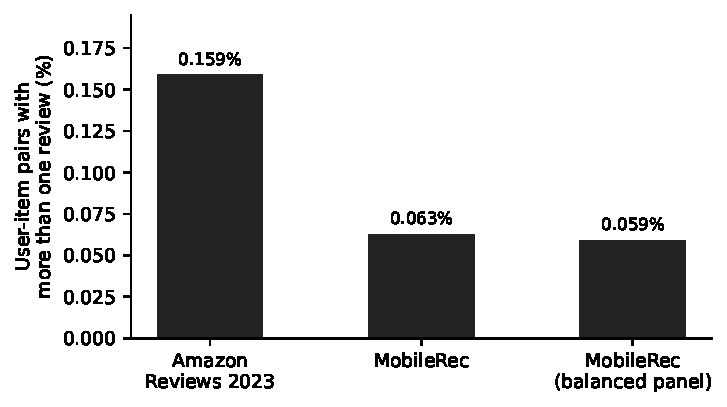
\includegraphics[width=0.66\textwidth]{figures/fig13_repeat_rates.pdf}
\caption{Share of user--item pairs carrying more than one review. Neither
corpus approaches the level a cohort analysis requires.}
\label{fig:repeat}
\end{figure}

This forecloses the analysis that motivated the study. If sentiment toward a
unit returns after a shock, that return may be because the reviewers who
complained changed their assessment, or because they left and different people
arrived. These have opposite managerial implications and are empirically
indistinguishable without repeat observations of the same individual. Any
recovery reported on such data is population-level, and the distinction is not
a refinement but a limit on what the measurement can mean.

\subsection{Aggregation restores density but not identifiability}

Aggregating to app category raised the qualifying share to 77.8\,\%. That
figure recomputes category membership each month, so it may reflect apps
entering and leaving rather than sentiment change. We therefore constructed
balanced panels retaining only apps present across a minimum share of the
window (Figure~\ref{fig:attrition}).

\begin{figure}[htbp]
\centering
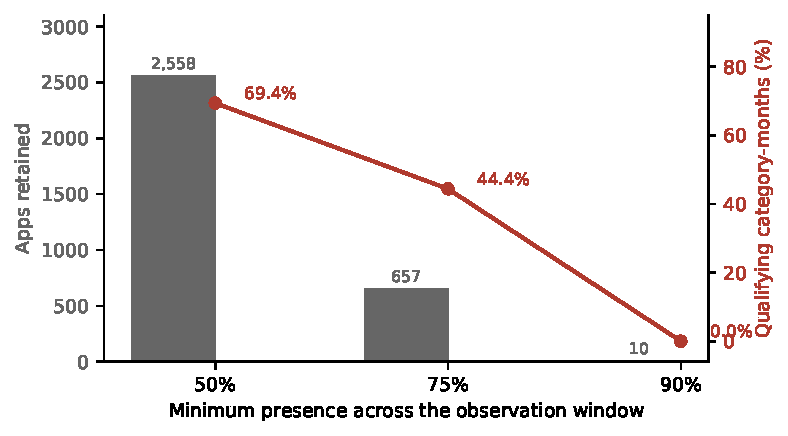
\includegraphics[width=0.72\textwidth]{figures/fig2_panel_attrition.pdf}
\caption{Apps retained and qualifying category-months as the presence
requirement tightens. Density survives at 75\,\% presence but collapses at
90\,\%, indicating that composition is not fully stable even in the balanced
panel.}
\label{fig:attrition}
\end{figure}

At 75\,\% presence, 657 apps and 46 categories survived, with 955 category-
months qualifying out of 2{,}150 category-months present in that panel, a share
of 44.4\,\% (95\,\% CI [42.3, 46.5], Wilson). The denominator is now logged.
An earlier version of this paper quoted the share without it and, worse, once
recovered a denominator by dividing the count by the share and reported the
result as measured; the logged figure is 2{,}150 and the derived one was
2{,}151. Compared against the 77.8\,\% obtained without balancing over
the same window, this is a relative reduction of 43\,\%:
composition change contributes materially to the apparent density, and roughly
two of every five qualifying category-months in the unbalanced figure depend on
apps that are not present throughout. Density survives balancing, but not
untouched, and the unbalanced figure should not be quoted as though it
described a stable panel. At 90\,\% presence only 10 apps remained and no
category-month qualified at all, which sets a firm limit on how far the
balanced-panel result can be pushed.

Shock detection requires 26 consecutive qualifying months (six baseline, two
shock, eighteen horizon). Sixteen categories met this criterion, with the
longest runs reaching 43 months (Figure~\ref{fig:runs}).

\begin{figure}[htbp]
\centering
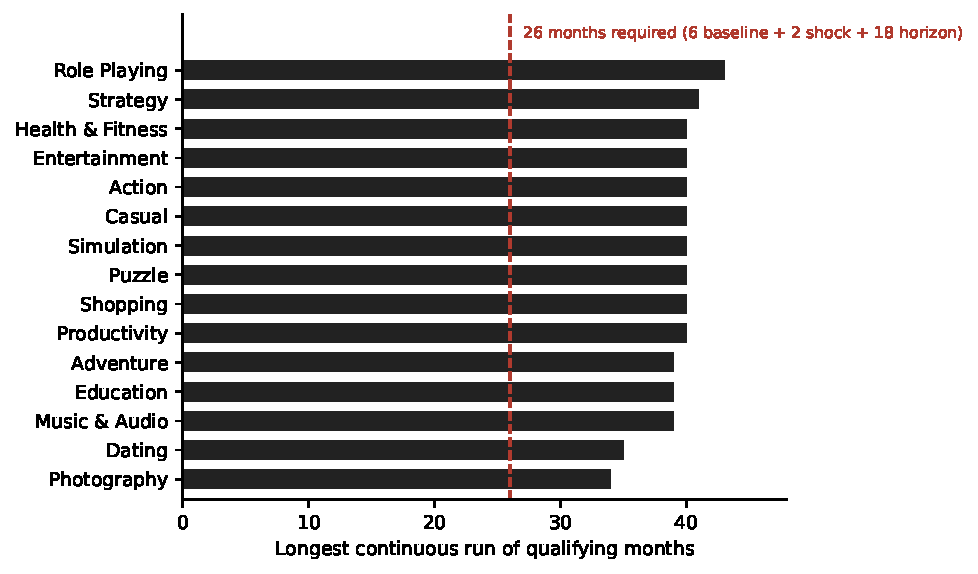
\includegraphics[width=0.78\textwidth]{figures/fig3_longest_runs.pdf}
\caption{Longest continuous run of qualifying months per category under the
75\,\% presence panel, against the 26 months a full shock-and-recovery window
requires. Top fifteen categories shown.}
\label{fig:runs}
\end{figure}

\subsection{Detected shocks are indistinguishable from noise}

Two counts must be distinguished here. Sixteen categories carry a run of 26 or
more contiguous qualifying months, long enough for a full shock-and-recovery
window. Detection, however, runs on any contiguous run longer than the baseline and
shock requirement combined. That requirement is $6 + 2 = 8$ months, and the
implementation admits runs \emph{exceeding} it, so the shortest usable run is
nine months: eight would leave no month in which recovery could be observed. A
category split by sparse months contributes more than one such run. That yields 27 usable series
across 46 categories. Series shorter than 26 months can host a shock but its
outcome is necessarily censored, which accounts for part of the censoring rates
below.

With that in hand, we ran detection on the 27 series under two sentiment
measures: mean star rating, which requires no model, and
lexicon polarity. Table~\ref{tab:outcomes} reports the results.

\begin{table}[htbp]
\centering
\caption{Shock detection outcomes and null comparison, balanced panel at
75\,\% presence. The star-rating column carries the reported result: it is
computed from the rating field alone and requires no extraction model and no
annotation. The lexicon column is a robustness check on an unvalidated measure
(Section~\ref{sec:limitations}) and is shown for comparison only; no conclusion
in this paper rests on it.}
\label{tab:outcomes}
\small
\begin{tabular}{@{}lrr@{}}
\toprule
 & \textbf{Star rating} & \textbf{Lexicon polarity} \\
 & \textit{(primary)} & \textit{(robustness only)} \\
\midrule
\multicolumn{3}{@{}l}{\textit{Detection}} \\
Usable category series & 27 & 27 \\
Shock episodes & 23 & 29 \\
\quad recovered & 20 & 12 \\
\quad non-recovered & 0 & 7 \\
\quad censored & 3 & 10 \\
Censoring rate & 13.0\,\% & 34.5\,\% \\
Analysable episodes & 20 & 19 \\
EPP (3 parameters) & 6.7 & 6.3 \\
EPP (6 parameters) & 3.3 & 3.2 \\
\addlinespace
\multicolumn{3}{@{}l}{\textit{Null comparison}} \\
Block bootstrap null (mean) & 28.39 & 26.19 \\
Block bootstrap null (SD) & 3.77 & 3.73 \\
Observed / block null & 0.81 & 1.11 \\
Empirical $p$ & 0.95 & 0.25 \\
Ratio 95\,\% CI & [0.64, 1.15] & [0.83, 1.53] \\
\bottomrule
\end{tabular}
\end{table}

We read the null comparison from the star-rating measure alone. Under star
ratings, 23 shocks were observed against $28.39 \pm 3.77$ expected under the
block bootstrap null at 999 replicates, a ratio of 0.81 with empirical
$p = 0.95$: \emph{fewer} events than noise produces. Under lexicon polarity, 29
were observed against $26.19 \pm 3.73$, a ratio of 1.11 with $p = 0.25$. These $p$-values are empirical
quantiles of the 999-replicate bootstrap distribution under the $(b+1)/(B+1)$
convention. An earlier version of this paper reported normal approximations
computed from 30 replicates; those values, $p = 0.91$ and $p = 0.25$, are
close to the empirical ones but are superseded.
Figure~\ref{fig:nulldist} places each observation within its null density.

\begin{figure}[htbp]
\centering
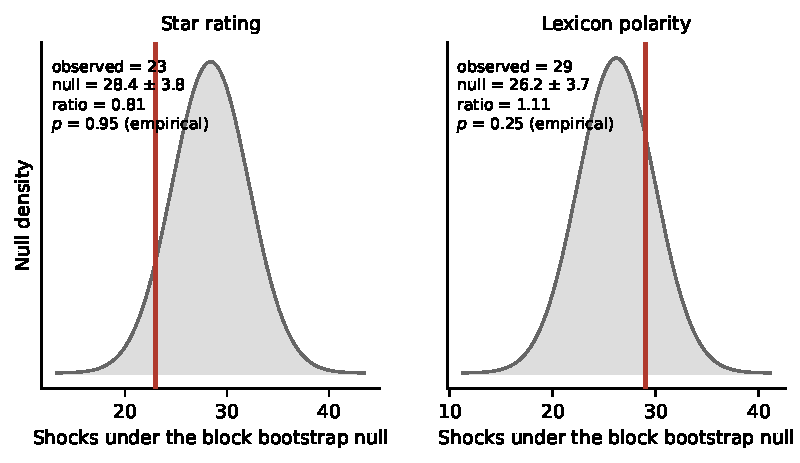
\includegraphics[width=0.88\textwidth]{figures/fig8_null_distributions.pdf}
\caption{Observed shock counts (vertical lines) against the block bootstrap
null density for each sentiment measure. Both observations fall inside the
bulk of the null distribution; the star-rating count falls below the null
mean.}
\label{fig:nulldist}
\end{figure}

\subsection{Does the instrument work? A positive control}
\label{sec:poscontrol}

A null result is uninformative unless the detector is shown to detect. Every
test written for this study checks classification logic: that a truncated
decline is censored, that a gap splits a series. None measures whether the
criterion recovers a shock that is actually present. We therefore ran a
positive control, injecting falls of known magnitude and duration into AR(1)
series matched to the observed panel in length, level and autocorrelation, and
measuring how often the criterion recovers them.

The synthetic geometry is stated rather than claimed to be matched. Series are
40 months long, which is the modal length of the qualifying runs in
Figure~\ref{fig:runs} but not their range, which spans nine to 43 months. The
level is 4.0 on the five-point rating scale and the innovation standard
deviation 0.10. Autocorrelation is set at $\phi = 0.6$, a moderate value we
chose rather than estimated from the panel. Power is reported against $\phi$ in
the repository output and falls from 0.89 at $\phi = 0$ to 0.59 at
$\phi = 0.85$ for a two-standard-deviation shock, so the figure we report sits
in the middle of that range rather than at its favourable end. The one
quantity we can check against the data is the false positive rate, and it
agrees with the observed bootstrap null; that agreement is the evidence that
the synthetic series are not unrepresentative.

The result is not favourable to our instrument and we report it in full
(Table~\ref{tab:poscontrol}).

\begin{table}[htbp]
\centering
\caption{Detection power of the pre-specified criterion on synthetic AR(1)
series: 27 series of 40 months at $\phi = 0.6$, one injected shock each, so
each cell rests on 27 trials and carries a standard error of roughly 0.09.
Differences of one or two cells are therefore not interpretable, and the
non-monotonicity at 0.5 SD should be read as noise. Power is the share of
injected shocks recovered within two months of their true onset. The false
positive column counts clean series, with nothing injected, on which the
criterion nonetheless fires.}
\label{tab:poscontrol}
\small
\begin{tabular}{@{}lrrrr@{}}
\toprule
\textbf{Injected shock} & \textbf{2 months} & \textbf{3 months} &
\textbf{6 months} & \textbf{False positives} \\
\midrule
0.5 SD & 0.56 & 0.44 & 0.56 & 1.00 \\
1.0 SD & 0.56 & 0.48 & 0.67 & 1.00 \\
1.5 SD & 0.56 & 0.59 & 0.70 & 1.00 \\
2.0 SD & 0.63 & 0.67 & 0.74 & 1.00 \\
3.0 SD & 0.70 & 0.78 & 0.89 & 1.00 \\
\bottomrule
\end{tabular}
\end{table}

Two things follow, and the second matters more than the first.

At its own criterion, a fall of one standard deviation sustained two months,
the rule recovers 56\,\% of injected shocks. At three standard deviations
sustained six months it reaches 89\,\%. Power rises with shock size, as it
must, but slowly: a sixfold increase in magnitude buys thirty percentage
points. The instrument discriminates weakly.

The false positive rate is 1.00. Every clean series, containing no injected
shock at all, produces at least one detection. This is not a defect discovered
late; it is the quantitative form of what the block bootstrap null was already
telling us. The null mean of 28.39 detections across 27 series is 1.05 per
series, and the synthetic control gives 1.00 per series. The two agree, which
is also a check that the synthetic series resemble the real ones.

The consequence for our claims is direct. We cannot say a shock would have been
found had one existed, because at realistic magnitudes the criterion finds
roughly two-thirds of them. And our observed count of 23 across 27 series, or
0.85 per series, is \emph{below} what the criterion produces on noise. The null
comparison is therefore correct in what it reports and cannot support the
stronger reading that the data contain no events. A criterion with a unit false
positive rate can only ever say that the data are not noisier than noise.

We report this rather than removing the criterion because it was
pre-specified, because its failure mode is informative for anyone adopting a
similar rule, and because the change point analysis that follows does not share
it.

\subsection{Change point detection finds what the threshold rule does not}
\label{sec:pelt}

The protocol named PELT as a robustness check on shock localisation. An earlier
version of this paper argued the check was moot because detection had already
failed against the null. That argument was wrong, and the run shows why: the
null comparison counts events, PELT locates them, and the two questions have
different answers.

On the same 27 category series under star ratings, PELT identified six change
points against $1.77 \pm 1.35$ expected under the same block bootstrap null:
a ratio of 3.40, $z = 3.15$, empirical $p = 0.015$. Under the threshold rule the
same series gave a ratio of 0.81 with $p = 0.95$.

\begin{table}[htbp]
\centering
\caption{Two detection procedures on identical series, each against the same
circular block bootstrap null at 999 replicates. The disagreement is the
result, not an inconsistency: the threshold rule asks how many sustained falls
of a given magnitude occur, and PELT asks where the mean shifts.}
\label{tab:pelt}
\small
\begin{tabular}{@{}lrrrr@{}}
\toprule
& \multicolumn{2}{c}{\textbf{Star rating}} & \multicolumn{2}{c}{\textbf{Lexicon}} \\
\cmidrule(lr){2-3}\cmidrule(lr){4-5}
& \textbf{Threshold} & \textbf{PELT} & \textbf{Threshold} & \textbf{PELT} \\
\midrule
Observed          & 23    & 6     & 29    & 1     \\
Null mean         & 28.39 & 1.77  & 26.19 & 0.80  \\
Null SD           & 3.77  & 1.35  & 3.73  & 0.86  \\
Ratio             & 0.81  & 3.40  & 1.11  & 1.26  \\
Empirical $p$     & 0.95  & 0.015 & 0.25  & 0.56  \\
\bottomrule
\end{tabular}
\end{table}

Three qualifications belong with this result and none of them is a reason to
set it aside.

The lexicon measure does not reproduce it: one change point against 0.80
expected, $p = 0.56$. Two measures of the same series again disagree, as they
did on outcome composition, and we cannot say which is right.

Six events across 27 series is a small number. The significance rests on the
null being small too, and a null mean below two makes the normal approximation
uncomfortable, which is why we report the empirical $p$.

The PELT penalty, $3\log(n)\sigma^2$, is a convention we adopted rather than
tuned, and change point counts are sensitive to it. A penalty chosen to produce
this result would be indefensible; we did not choose it that way, but neither
did we test alternatives, and a confirmatory study should.

A fourth qualification is decisive and we state it plainly. Four tests were run
on the same 27 series against the same null: two procedures crossed with two
sentiment measures. Under Bonferroni correction across that family,
$p = 0.015$ becomes $p_{\mathrm{adj}} = 0.060$, and the PELT result no longer
reaches conventional significance. An earlier version of this paper asserted
that multiple comparison correction "would only strengthen the reported
conclusion", which was true when every test was null and ceased to be true the
moment one was not. We have no principled argument for treating these four as
separate families, since they share a dataset, a null and a research question.

What we take from the result is therefore narrower than a positive finding.
Category-level star rating series show temporal structure that is suggestive
against a block bootstrap null and does not survive correction for the number
of tests performed. Our pre-specified event criterion does not capture that
structure at all. We report the uncorrected and corrected values together and
draw no conclusion from either.

\subsection{Two findings, at two different levels}
\label{sec:twolevels}

Before the aspect analysis we separate two results that are easy to merge and
should not be.

The first is that whole-review sentiment at category level produces shock
counts indistinguishable from noise. That is a statement about
\emph{category-level, whole-review} sentiment, measured on the star rating.

The second is that aspect-level series do not form at all. That is a statement
about \emph{density}, and it is logically prior: where no series exists, no
null comparison is possible.

Our title concerns the second. The first is reported because it is what the
data permitted and because it bears on the wider literature, not because it
establishes anything about aspects. A reader should not take the null result as
evidence about aspect-level recovery; the evidence about aspect-level recovery
is that it cannot be attempted.

\subsection{Aspect-level series do not form at all}
\label{sec:aspect}

The analyses above measure sentiment over whole reviews. That is
category-level sentiment, and a study about attributes cannot rest on it. We
therefore applied the aspect taxonomy to the same balanced panel and rebuilt
the series as (category, aspect, month).

Splitting 74{,}780 reviews across 46 categories, 10 aspects and 48 months gives
22{,}080 possible cells, of which 7{,}084 were non-empty (32.1\,\%), at a
median of one mention each.
\textbf{None reached the 30-mention threshold, and no aspect series survived to
be tested.} Figure~\ref{fig:aspectdens} gives the breakdown: performance and
design form the most cells but still carry a median of two mentions; delivery,
the sparsest, forms 165 cells at a median of one.

\begin{figure}[htbp]
\centering
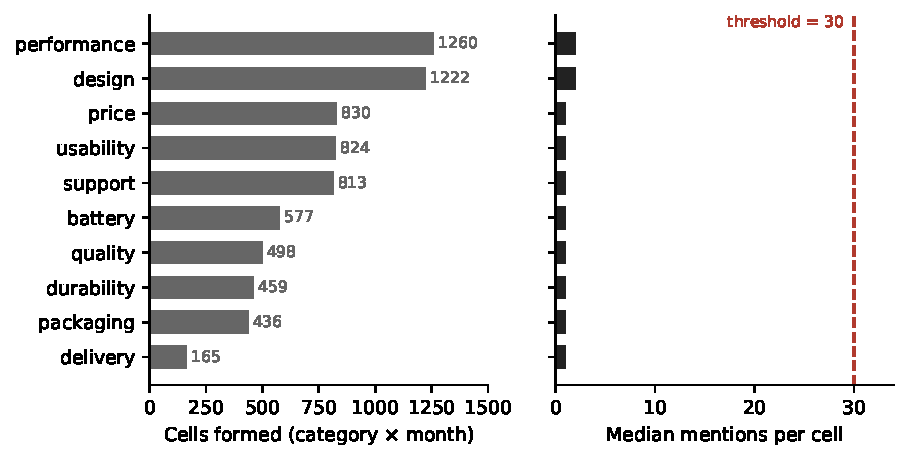
\includegraphics[width=0.88\textwidth]{figures/fig11_aspect_density.pdf}
\caption{Aspect cells formed on the balanced panel (left) and their median
mention count against the threshold (right). No aspect approaches it.}
\label{fig:aspectdens}
\end{figure}

\subsection{A bound independent of the extractor}
\label{sec:bound}

Our lexicon was built for physical products and maps imperfectly onto apps:
\emph{delivery} and \emph{packaging} mean little for software. Low coverage
could therefore reflect a domain mismatch rather than sparsity, and that
objection cannot be met by defending the lexicon.

It can be met by arithmetic. Let $R$ be the mean reviews per unit-period, $m$
the mean number of aspects a review mentions, and $T$ the mention threshold.
Total mentions available per unit-period is at most $Rm$, so the number of
aspects $j$ that can simultaneously reach $T$ satisfies
\begin{equation}
j \;\leq\; \frac{Rm}{T}.
\label{eq:bound}
\end{equation}

This does not assume even distribution. Skewed extraction concentrates
mentions, which can lift one aspect above the threshold, but it cannot raise
the total: whatever one aspect gains another loses. Equation~\ref{eq:bound}
therefore bounds how many aspects can qualify under any assignment, uniform or
not. It is an upper bound and not an estimate: the realised number may be lower
and never higher, and under strong skew it can be zero even where the bound
permits one.

For the balanced MobileRec panel, $R = 74{,}780 / 2{,}150 = 34.8$ and $T = 30$.
Even at $m = 1$ the bound gives $j \leq 1.16$, so at most one aspect of any
taxonomy can qualify; at $m = 3$, at most three. An earlier version of this
paper used $R = 33.9$, dividing by the $46 \times 48 = 2{,}208$ maximum rather
than the 2{,}150 category-months the panel contains. The logged denominator is
the correct divisor and the figures here use it. A ten-aspect study is infeasible unless reviews
mention nine aspects each. Under the even-distribution case the shortfall is
starker still: expected mentions per cell is $34.8/k$, meeting the threshold
only at $k = 1$, falling to 17.4 at $k = 2$ and 3.5 at $k = 10$
(Figure~\ref{fig:ceiling}).

The Amazon extract fails the bound more decisively. Its 82{,}041 reviews span
11{,}925 product-months, or $R = 6.9$ reviews per product-month. At $m = 1$ the
bound gives $j \leq 0.23$: not one aspect can qualify, and the shortfall is a
factor of 4.4 before any aspect split is applied at all. This is why no
aspect-level analysis was attempted on Amazon. It would have been arithmetic
performed on an empty set.

\begin{figure}[htbp]
\centering
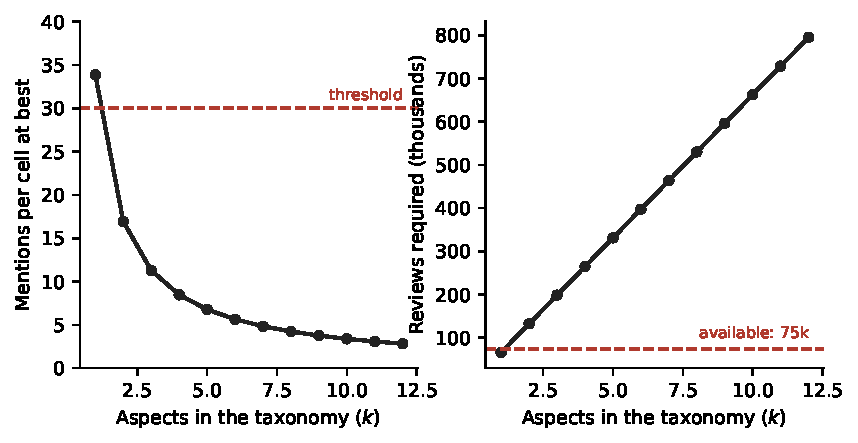
\includegraphics[width=0.88\textwidth]{figures/fig12_ceiling.pdf}
\caption{Best-case mentions per cell (left) and reviews required for full
coverage (right) against taxonomy size $k$. Required reviews are
$30k \times 46 \times 48$ at $m = 1$; at $k = 10$ this is 662{,}400. The
reference line marks the 74{,}780 reviews the balanced panel holds. The bound
assumes an extractor that never misses and never over-assigns, so no real
extractor can do better.}
\label{fig:ceiling}
\end{figure}

Two parameters govern the bound and neither was measured. We report both
rather than fixing them silently.

The first is $m$. We never estimated the mean number of aspects a review names,
because our lexicon was not validated and an unvalidated extractor cannot
estimate it. Every statement above is therefore conditional on $m$, and where
we write a single number we have set $m = 1$. That is the conservative choice
for our argument only in the sense that it is the smallest defensible value; it
is not a measurement, and a reader should treat $j \leq 1.16m$ rather than
$j \leq 1.16$ as the result.

The second is $T$. Table~\ref{tab:threshold} gives the bound across thresholds.
The conclusion is not threshold-free: at $T = 30$ the MobileRec panel supports
at most $1.16m$ aspects, but at $T = 10$ it supports $3.48m$, so a ten-aspect
taxonomy becomes arithmetically possible once $m \geq 3$. What the table shows
is the combination required, and we make no claim beyond it.

\begin{table}[htbp]
\centering
\caption{The density bound $j \leq Rm/T$ across mention thresholds, for the
MobileRec balanced panel ($R = 34.8$) and the Amazon extract ($R = 6.9$).
Entries are coefficients on $m$: the maximum number of aspects that can reach
the threshold is the entry multiplied by the mean aspects named per review.
Amazon fails at every threshold we would consider defensible.}
\label{tab:threshold}
\small
\begin{tabular}{@{}lrrrrrr@{}}
\toprule
\textbf{Threshold $T$} & 5 & 10 & 15 & 20 & 30 & 50 \\
\midrule
MobileRec, category & 6.96$m$ & 3.48$m$ & 2.32$m$ & 1.74$m$ & 1.16$m$ & 0.70$m$ \\
Amazon, product     & 1.38$m$ & 0.69$m$ & 0.46$m$ & 0.35$m$ & 0.23$m$ & 0.14$m$ \\
\bottomrule
\end{tabular}
\end{table}

A low threshold is not free. At $T = 5$ a monthly cell mean rests on five
mentions, and the shock criterion compares such a mean against a standard
deviation estimated from six of them. We fixed $T = 30$ before seeing data for
that reason, and we do not revisit it now; but the honest statement is that our
negative conclusion holds at the threshold we pre-specified and weakens as the
threshold falls.

The bound holds whatever the extraction method, because no extractor can
recover an attribute judgement from a review that was never written. An
aspect-level study of recovery on this corpus is not limited by method but by
how much text exists.

This is the appropriate answer to the natural objection that a transformer or
instruction-tuned model would extract more than a lexicon. It would, and we do
not dispute it. A better extractor raises $m$, the mean aspects recovered per
review, and Equation~\ref{eq:bound} is linear in $m$. Reaching ten qualifying
aspects on the MobileRec panel would require $m \geq 8.6$: every review would
have to yield judgements on close to nine distinct attributes. Reaching even
three would require $m \geq 2.6$. These are not extraction targets; they are
statements about how much is said in a typical app review. We did not run a
transformer baseline for this reason, and we state the omission plainly rather
than implying it was unnecessary: a reviewer who believes $m \geq 3$ is
attainable on short app reviews should regard this part of our argument as
untested.

\subsection{Time to recovery}
\label{sec:km}

With the episodes classified, a Kaplan--Meier estimate of time to recovery is
available and we report it rather than describing why we did not.

Under star ratings the median time to recovery is three months, with the
survival curve falling to zero by month 14 and no episode reaching the
18-month horizon uncovered. Under lexicon polarity the median is 15 months and
the curve does not reach zero. A five-fold difference between two measures of
the same episodes is not a result about recovery; it is further evidence that
the episodes are not stable objects.

Confidence bands are wide throughout, as 23 and 29 episodes require. We fit no
Cox model: at 20 and 19 analysable episodes the events-per-parameter figures in
Table~\ref{tab:outcomes} rule it out, and a hazard ratio estimated from them
would carry a precision the data cannot support.

\subsection{What the null comparison could have detected}
\label{sec:nullpower}

A null comparison that fails to reject is uninformative unless its own
sensitivity is stated. Treating the bootstrap null as approximately normal, the
one-sided critical value at $\alpha = 0.05$ is 33.7 shocks for star ratings and
33.2 for lexicon polarity, ratios of 1.21 and 1.28. At 80\,\% power the
smallest detectable ratios are 1.32 and 1.42.

Our result therefore rules out a signal inflating shock counts by roughly a
third or more above chance. It does not rule out a smaller one, and we claim no
such thing. Detecting a 10\,\% excess at this null variance would need about an
order of magnitude more series than the 27 available, which returns the problem
to the density constraint of Section~\ref{sec:results}.

\subsection{The two measures disagree}
\label{sec:disagree}

Star ratings produced no non-recovered episode, while lexicon polarity produced
seven. An earlier version of this paper offered the divergence as evidence that
the episodes were not real events. That inference does not hold. A mean star
rating is an overall judgement and a lexicon score is a property of review
text; they are not two measurements of one construct, and divergence between
them is expected rather than diagnostic. We report the difference as a
description of the two measures and draw no inference from it.

The comparison retains one use. The star-rating measure requires no model and
no annotation, so a reader who distrusts the unvalidated lexicon can read every
reported conclusion from the star-rating column alone. Nothing in this paper
depends on the lexicon.

Figure~\ref{fig:disagree} shows the outcome composition under each measure. We display it because the two columns of Table~\ref{tab:outcomes} invite the comparison, not because the difference supports an inference; for the reason given above, it does not.

\begin{figure}[htbp]
\centering
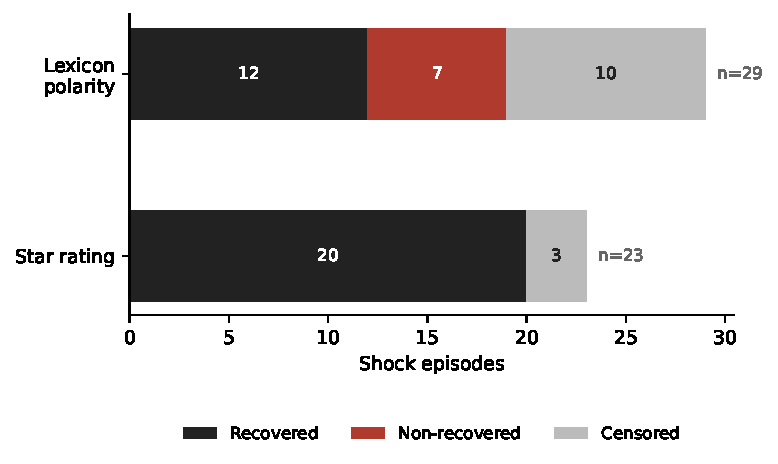
\includegraphics[width=0.72\textwidth]{figures/fig6_measure_disagreement.pdf}
\caption{Outcome composition on identical series: 23 episodes under star
rating, 29 under lexicon polarity. Star ratings produced no non-recovered
episode; see Section~\ref{sec:disagree} for why that is not interpretable on
its own.}
\label{fig:disagree}
\end{figure}

\subsection{Sensitivity}

Figure~\ref{fig:sensitivity} reports shock counts across the detection
parameter grid. Counts fall monotonically as either the magnitude threshold or
the duration requirement is tightened, as expected, and no cell yields a count
that would change the power conclusion. We note that relaxing thresholds until
events appear would be the natural response to these results and would be
invalid: events recovered that way are the noise the null comparison already
identifies.

\begin{figure}[htbp]
\centering
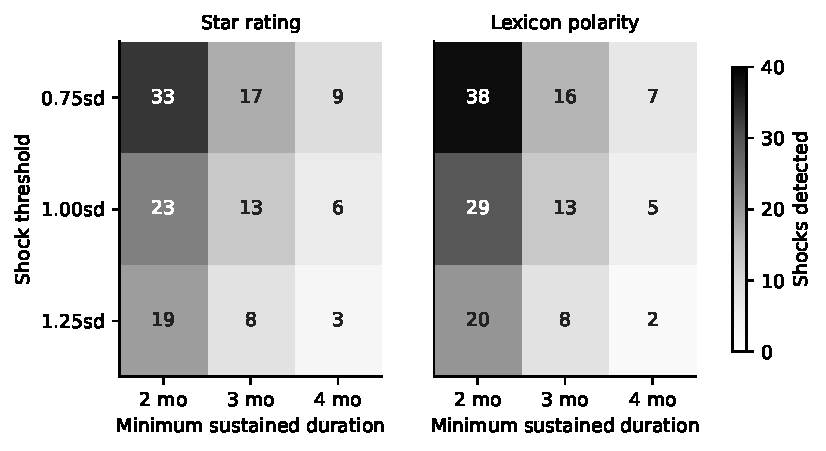
\includegraphics[width=0.85\textwidth]{figures/fig5_sensitivity.pdf}
\caption{Shocks detected across the detection parameter grid for both measures.
Counts fall monotonically as either criterion tightens; no cell yields a count
that would change the power conclusion, and none was significant against the
null.}
\label{fig:sensitivity}
\end{figure}

\subsection{Methodological controls and what each prevents}

Table~\ref{tab:controls} lists the controls and the specific failure mode each
addresses. Seven were implemented and exercised, each with an automated test asserting its
behaviour on a synthetic case with a known correct answer. The last of them,
the positive control of Section~\ref{sec:poscontrol}, was added after an earlier
version of this paper was reviewed and is the one that most changed what we
could claim. One control was specified in the protocol but never exercised,
because the analysis it guards was never reached; they are marked accordingly, and we
list them because the failure modes they describe apply to any study that does
reach those analyses.

\begin{table}[htbp]
\centering
\caption{Controls implemented, the artefact each prevents, and the direction
of the bias if the control is omitted.}
\label{tab:controls}
\small
\begin{tabular}{@{}p{2.9cm}p{6.0cm}p{4.4cm}@{}}
\toprule
\textbf{Control} & \textbf{Failure mode prevented} & \textbf{Direction of
omitted-control bias} \\
\midrule
\multicolumn{3}{@{}l}{\textit{Implemented and exercised}} \\[2pt]
Right-censoring of short follow-up
& Shocks near the end of the window cannot be observed to recover
& Overstates irreversibility; grows with the horizon \\[3pt]
Circular block bootstrap null
& Permutation removes autocorrelation and raises the detection threshold
& Understates the null; favours detection \\[3pt]
Cohort vs population recovery
& A returning average may reflect new reviewers, not changed minds
& Attributes turnover to perceptual recovery \\[3pt]
Gap-aware segmentation
& Series with dropped months are otherwise treated as contiguous
& Creates spurious shocks across discontinuities \\[3pt]
Balanced panel
& Category membership recomputed each month conflates composition with level
& Attributes composition change to sentiment change \\[3pt]
Guarded ratio reporting
& Recovery attribution is unstable when the denominator approaches zero
& Emits plausible but meaningless ratios \\[3pt]
Positive control
& A detector may fail silently on shocks that are present
& Would let a null result be read as evidence of absence \\[5pt]
\multicolumn{3}{@{}l}{\textit{Specified but never exercised}} \\[2pt]
Time-varying recovery covariate
& Recovery status requires survival to be observed, creating immortal time
& Manufactures a protective effect of recovery \\
\bottomrule
\end{tabular}
\end{table}

\subsection{A note on dataset provenance}

The Amazon Reviews 2023 collection pipeline is user-centric: user identifiers
are sampled first, and all review pages associated with each sampled user are
then retrieved. The authors note that item-level review coverage may be
incomplete when some reviewers of an item fall outside the user
pool~\citep{hou2026}. This is appropriate for the recommendation tasks the
dataset targets, but it means item-level series are thinned by construction,
independently of how often customers review. Our product-level density figures
should therefore be read as a property of this corpus as well as of reviewing
behaviour. Both corpora we examined are sampled user-centrically, and we did not survey
others. We make no claim about what public corpora exist: a systematic review
of candidates such as Yelp, Goodreads, Steam or TripAdvisor against the
requirements in Section~\ref{sec:whatdata} would be a useful exercise and we
have not performed it. What we can say is that neither corpus we used provides
item-complete longitudinal coverage, and that an item-centrically sampled
corpus would remove one of the two constraints described above, leaving the
behavioural one intact.

Table~\ref{tab:provenance} sets out the properties each corpus offers against
what the design requires.

\begin{table}[htbp]
\centering
\caption{Design requirements against corpus properties. A requirement is met
only if it holds at the unit of analysis the design uses. \textit{n.t.}: not
tested, because the configuration failed an earlier requirement and the step was
never reached. For Amazon specifically, no aspect extraction was attempted
because the density bound of Section~\ref{sec:bound} rules out any aspect
reaching the threshold at $R = 6.9$, before extraction quality enters.}
\label{tab:provenance}
\small
\begin{tabular}{@{}p{5.0cm}ccc@{}}
\toprule
\textbf{Requirement} & \textbf{Amazon 2023} & \textbf{MobileRec (app)} &
\textbf{MobileRec (category)} \\
\midrule
Timestamped reviews & yes & yes & yes \\
Persistent user identifier & yes & yes & yes \\
$\geq$ 30 mentions per unit-month & 2.6\,\% & 0.2\,\% & 44.4\,\% \\
$\geq$ 26 contiguous qualifying months & no & no & 16 categories \\
Repeat review of the same item & 0.16\,\% & 0.06\,\% & 0.06\,\% \\
Aspect cells above threshold & n.t. & n.t. & 0 of 7{,}084 \\
Signal above block bootstrap null & n.t. & n.t. & no \\
Documented intervention dates & no & no & no \\
\bottomrule
\end{tabular}
\end{table}

\section{Discussion}

\subsection{The obstacle is behavioural}

Three configurations failed for three different proximate reasons: density,
repeat observation, and signal-to-noise. Two causes compound. Most reviewers
write once and do not return, which is a property of behaviour. And the
corpora available at this scale are assembled user-centrically, which thins
item-level series further~\citep{hou2026}. The first cause cannot be
engineered away by choosing a different corpus; the second could be, but we
are not aware of a public corpus that does so at the required scale. Choosing a
third corpus with the same behavioural profile and the same sampling design
would reproduce the result; an item-centrically sampled corpus would relieve
the second constraint but not the first.

\subsection{A test others can apply before committing}

The bound in Section~\ref{sec:bound} is arithmetic and transfers. Before
designing an aspect-level temporal study, divide the reviews available in the
intended panel by (units $\times$ periods $\times$ aspects) and compare against
whatever mention threshold the analysis needs. If the quotient falls short, no
choice of extractor or model will rescue the design, and the remedy is more
text or coarser time periods rather than a better method. We claim nothing for the
inequality itself, which is elementary. We claim only that computing it before
assembling a panel is not standard practice and that stating it in a form that
transfers has some use as a first step in study design. We did not compute it
first, which is why this paper exists.

\subsection{What data would make this estimable}
\label{sec:whatdata}

Inverting Equation~\ref{eq:bound} turns the negative result into a
specification. For a study of $j$ aspects at threshold $T$ over $P$ periods and
$U$ units, the corpus must supply at least $UPjT/m$ reviews, and they must be
distributed across units and periods rather than concentrated at launch. For a
modest design of five aspects, monthly periods over three years, fifty units
and $T = 30$ at $m = 2$, that is 135{,}000 reviews \emph{within the panel},
or 1.8 times the balanced panel we assembled from a corpus of 19.3 million
interactions.

Three further properties are needed and none of them follows from volume.
Repeat observation of the same user on the same item, at a rate high enough to
estimate a cohort, is required to separate perceptual recovery from turnover;
neither corpus here comes within two orders of magnitude. Item-centric rather
than user-centric sampling is required so that item series are not thinned by
construction. Item-centric sampling matters in both corpora studied here, not only in
Amazon: MobileRec's 5-core filter is applied to users, so items reviewed by
few sampled users are thinned in the same way. And documented intervention
dates are required if recovery is to be attributed to anything: without them the analysis can describe when
sentiment moved but never why.

We suspect such data exists inside firms and not outside them. That is a
limitation of public corpora rather than of the construct, and it suggests that
progress on recovery dynamics will come from industry collaboration or from
purpose-built collection, not from re-mining the corpora already available.

\subsection{Implications for recovery claims}

Our findings do not show that sentiment recovery does not occur. They show
that on public review data it is not identifiable in the way the construct
requires. Two consequences follow for work that reports recovery-like
patterns.

First, in the absence of repeat individual observation, a returning average is
consistent with perceptual recovery and with population turnover, and these
cannot be told apart. Reporting the former without excluding the latter
overstates what the data support.

Second, results at aggregated levels require an explicit null. Our category
series were dense enough to produce plausible shock counts with plausible
recovery patterns; only the block bootstrap comparison revealed that these
were not distinguishable from noise. A study reporting
Table~\ref{tab:outcomes} without its lower panel would appear to have found
something.

\subsection{Null choice is not a detail}
\label{sec:nullchoice}

As shown in Section~\ref{sec:nulls}, the permutation null is biased toward the
alternative because it removes the autocorrelation that sets the detection
threshold. Under star ratings the permutation null returned 25.8 against the
block bootstrap's 27.8; the direction of the bias matches our synthetic
demonstration. Studies of temporal review dynamics that validate against
permutation nulls, or against no null at all, may be reporting detection rates
that a suitable control would not support.

\section{Limitations}
\label{sec:limitations}

Our search of the prior literature was targeted rather than systematic, so we
cannot claim the gap identified in Section~\ref{sec:gap} is unoccupied; a search conducted and reported under PRISMA \citep{page2021, moher2009}
would be required. Our analyses use
subsamples of both corpora rather than their full extent, and a larger extract
could change the density figures, though it would not change the repeat-review
rate, which is a property of behaviour rather than sample size. The lexicon used for polarity is deliberately crude, and we must be explicit
about what was not done. Its weakness bears on
Section~\ref{sec:aspect} but not on Section~\ref{sec:bound}, whose bound is
independent of the extractor. Our protocol specified validation of extraction against 300
human-labelled reviews, with agreement reported as Cohen's $\kappa$. That
validation was never carried out, because the feasibility constraints in
Section~\ref{sec:results} made the downstream analysis moot before annotation
was reached. The lexicon measure is therefore unvalidated and any inference resting
on it alone should be discounted accordingly; we report it only alongside the
star-rating measure, which requires no model and no annotation, and which
produced the weaker of the two null ratios. A trained aspect-based model might
detect structure our measure misses, and that possibility is not excluded here.

Four tests were run across two procedures and two sentiment measures on one set
of series. Bonferroni correction across that family is applied in
Section~\ref{sec:pelt} and changes the one suggestive result from
$p = 0.015$ to $p = 0.060$. We do not additionally correct across the 27
individual series, since no per-series result is reported.
Finally, the category-level analysis was exploratory: it was not covered by the protocol, and its
results are reported as exploratory.

We did not screen for coordinated review campaigns, which produce
shock-like signatures and are a known contaminant of review corpora. Opinion
spam was characterised by \citet{jindal2008} and \citet{ott2011}, group
manipulation by \citet{mukherjee2012}, and detection methods are surveyed by
\citet{mohawesh2021} and \citet{paul2021}. Manipulation has measurable
commercial value \citep{luca2011}, which is why it persists. Because our conclusion is that detected shocks are
indistinguishable from noise, undetected manipulation would if anything work
against that conclusion by adding real structure; screening would nevertheless
be required in any confirmatory analysis.

Two analyses specified in the protocol remain unrun. No Cox model was fitted,
because 20 analysable episodes fall an order of magnitude below what one needs;
Kaplan--Meier is reported instead (Section~\ref{sec:km}). And no transformer or
instruction-tuned extractor was compared against the lexicon, which matters more
than it did in earlier versions of this paper because the density bound is
stated in terms of $m$ and $m$ is unmeasured. A reader who believes a modern
extractor would raise $m$ substantially on short app reviews should treat
Section~\ref{sec:bound} as untested at that point.

Two others were unrun when an earlier version of this paper was written and have
since been carried out. The bootstrap now uses 999 replicates with empirical
$p$-values rather than 30 with a normal approximation. PELT was run, and its
result disagrees with the threshold rule (Section~\ref{sec:pelt}); we had
previously argued the check was unnecessary, and that argument was wrong.

We also note that a category-level shock is not the same phenomenon as a
product-level one. It averages hundreds of apps and may reflect store ranking
changes, operating system releases, or seasonal effects rather than perceptual
change. We did not attempt to separate these, because the null comparison made
the question moot.

\section{Conclusion}

We set out to model attribute-level sentiment decline and return as a
time-to-event process and found that the subsamples examined here cannot
support it. Two results, at two levels, should not be run together.

At the aspect level the series do not form: none of 7{,}084 cells reached the
mention threshold. The density bound explains why and says how far the
shortfall extends, at $j \leq 1.16m$ for the MobileRec panel and $0.23m$ for
the Amazon extract at $T = 30$. Because $m$ was never measured, this is a
conditional statement, and Table~\ref{tab:threshold} shows how it moves with
the threshold.

At category level, where whole-review sentiment does yield series, the result
is mixed and we resist resolving it. Our pre-specified event criterion found
shock counts indistinguishable from a block bootstrap null, at a ratio of 0.81.
PELT, applied to the same series against the same null, found change points at
a ratio of 3.40, $p = 0.015$ uncorrected and $p = 0.060$ under Bonferroni
across the four tests performed. Temporal structure is present in
category-level star ratings; our criterion does not recover it; and the lexicon
measure reproduces neither result. We report all three rather than selecting the one
that reads most cleanly.

This bears on the paper's scope. We can say that an aspect-level time-to-event
study is not possible on these corpora, and the density bound explains why in
terms that transfer. We cannot say that category-level review series are
structureless, and the PELT result is evidence that they are not. At the
product and app levels the series are one to two orders of magnitude too
sparse and the resulting event counts fall short of the required power by more
than an order of magnitude. Repeat reviewing of the same item is rare enough
that recovery of a population average cannot be separated from turnover in the
reviewing population. Aggregation to the category level restores density but
yields shock counts indistinguishable from a block bootstrap null under either
of two sentiment measures, which themselves disagree about outcomes.

We report this because the design is a natural one that others are likely to
attempt, because feasibility failures are systematically under-reported
\citep{franco2014}, and because the failure points are informative independently of our
particular hypotheses. The pre-specified definitions, the code, and the self-test suite are
available so that the assessment can be checked or
extended to other corpora.

\section*{Data and code availability}

All code, pre-specified definitions, self-tests, and figure generation
scripts: \url{https://github.com/ssvakil/aspect-recoverability}. Both datasets
analysed are publicly available from their original distributors.

\section*{Author contributions}

\textbf{S. Vakil:} conceptualisation, methodology, software, formal analysis,
data curation, writing --- original draft, visualisation.
\textbf{Y. Farjami:} supervision, methodology, writing --- review and editing.

\section*{Declaration of competing interests}

The authors declare no competing interests.

\FloatBarrier

\begin{thebibliography}{99}

% All entries below carry full bibliographic details obtained from an
% authoritative source (publisher page, PubMed, ACL Anthology, ACM DL,
% ScienceDirect) or from the reference list of a retrieved peer-reviewed
% document. Entries marked [check] should have volume and page numbers
% confirmed in Scopus or Web of Science before submission.

% ---------------- Datasets ----------------

\bibitem[Hou et al.(2026)]{hou2026}
Hou, Y., Li, J., Fu, X., He, Z., Yan, A., Chen, X., McAuley, J. (2026).
Bridging language and items for retrieval and recommendation: benchmarking
LLMs as semantic encoders. In \textit{Proceedings of the 64th Annual Meeting
of the Association for Computational Linguistics}, 3251--3265.

\bibitem[Maqbool et al.(2023)]{maqbool2023}
Maqbool, M.H., Farooq, U., Mosharrof, A., Siddique, A.B., Foroosh, H. (2023).
MobileRec: a large-scale dataset for mobile apps recommendation. In
\textit{Proceedings of the 46th International ACM SIGIR Conference on Research
and Development in Information Retrieval}, 3007--3016.

% ---------------- Attribute-level analysis of reviews ----------------

\bibitem[Hu and Liu(2004)]{hu2004}
Hu, M., Liu, B. (2004).
Mining and summarizing customer reviews. In \textit{Proceedings of the 10th
ACM SIGKDD International Conference on Knowledge Discovery and Data Mining},
168--177.

\bibitem[Xia et al.(2021)]{xia2021}
Xia, P., Jiang, W., Wu, J., Xiao, S., Wang, G. (2021).
Exploiting temporal dynamics in product reviews for dynamic sentiment
prediction at the aspect level.
\textit{ACM Transactions on Knowledge Discovery from Data}, 15(4),
Article 68, 1--29.

\bibitem[Maalej and Nabil(2015)]{maalej2015}
Maalej, W., Nabil, H. (2015).
Bug report, feature request, or simply praise? On automatically classifying app
reviews. In \textit{IEEE 23rd International Requirements Engineering
Conference}, 116--125.

\bibitem[Mittal et al.(1999)]{mittal1999}
Mittal, V., Kumar, P., Tsiros, M. (1999).
Attribute-level performance, satisfaction, and behavioral intentions over time:
a consumption-system approach.
\textit{Journal of Marketing}, 63(2), 88--101.

\bibitem[Park and Kim(2024)]{park2024}
Park, S., Kim, H. (2024).
Extracting product design guidance from online reviews: an explainable neural
network-based approach.
\textit{Expert Systems with Applications}, 236, 121357.

\bibitem[Roelen-Blasberg et al.(2023)]{roelen2023}
Roelen-Blasberg, T., Habel, J., Klarmann, M. (2023).
Automated inference of product attributes and their importance from
user-generated content: can we replace traditional market research?
\textit{International Journal of Research in Marketing}, 40(1), 164--188.

\bibitem[Yang et al.(2023)]{yang2023}
Yang, T., Dang, Y., Wu, J. (2023).
How to prioritize perceived quality attributes from consumers' perspective?
Analysis through social media data.
\textit{Electronic Commerce Research}. % [check] volume and pages

\bibitem[Zhou et al.(2023)]{zhou2023}
Zhou, L., Tang, L., Zhang, Z. (2023).
Extracting and ranking product features in consumer reviews based on evidence
theory.
\textit{Journal of Ambient Intelligence and Humanized Computing}, 14(8),
9973--9983.

% ---------------- Failure, recovery, negativity ----------------

\bibitem[Baumeister et al.(2001)]{baumeister2001}
Baumeister, R.F., Bratslavsky, E., Finkenauer, C., Vohs, K.D. (2001).
Bad is stronger than good.
\textit{Review of General Psychology}, 5(4), 323--370.

\bibitem[de Matos et al.(2007)]{dematos2007}
de Matos, C.A., Henrique, J.L., Rossi, C.A.V. (2007).
Service recovery paradox: a meta-analysis.
\textit{Journal of Service Research}, 10(1), 60--77.

\bibitem[LaBarbera and Mazursky(1983)]{labarbera1983}
LaBarbera, P.A., Mazursky, D. (1983).
A longitudinal assessment of consumer satisfaction/dissatisfaction: the dynamic
aspect of the cognitive process.
\textit{Journal of Marketing Research}, 20(4), 393--404.

\bibitem[Rozin and Royzman(2001)]{rozin2001}
Rozin, P., Royzman, E.B. (2001).
Negativity bias, negativity dominance, and contagion.
\textit{Personality and Social Psychology Review}, 5(4), 296--320.

% ---------------- Survival analysis ----------------

\bibitem[Cox(1972)]{cox1972}
Cox, D.R. (1972).
Regression models and life-tables.
\textit{Journal of the Royal Statistical Society: Series B}, 34(2), 187--220.

\bibitem[Kaplan and Meier(1958)]{kaplan1958}
Kaplan, E.L., Meier, P. (1958).
Nonparametric estimation from incomplete observations.
\textit{Journal of the American Statistical Association}, 53(282), 457--481.

\bibitem[Peduzzi et al.(1996)]{peduzzi1996}
Peduzzi, P., Concato, J., Kemper, E., Holford, T.R., Feinstein, A.R. (1996).
A simulation study of the number of events per variable in logistic regression
analysis.
\textit{Journal of Clinical Epidemiology}, 49(12), 1373--1379.

\bibitem[Schoenfeld(1983)]{schoenfeld1983}
Schoenfeld, D.A. (1983).
Sample-size formula for the proportional-hazards regression model.
\textit{Biometrics}, 39(2), 499--503.

\bibitem[van Smeden et al.(2016)]{vansmeden2016}
van Smeden, M., de Groot, J.A.H., Moons, K.G.M., Collins, G.S., Altman, D.G.,
Eijkemans, M.J.C., Reitsma, J.B. (2016).
No rationale for 1 variable per 10 events criterion for binary logistic
regression analysis.
\textit{BMC Medical Research Methodology}, 16, 163.

\bibitem[Vittinghoff and McCulloch(2007)]{vittinghoff2007}
Vittinghoff, E., McCulloch, C.E. (2007).
Relaxing the rule of ten events per variable in logistic and Cox regression.
\textit{American Journal of Epidemiology}, 165(6), 710--718.

% ---------------- Immortal time bias ----------------

\bibitem[Karim et al.(2016)]{karim2016}
Karim, M.E., Gustafson, P., Petkau, J., et al. (2016).
Comparison of statistical approaches for dealing with immortal time bias in
drug effectiveness studies.
\textit{American Journal of Epidemiology}, 184(4), 325--335.

\bibitem[L\'evesque et al.(2010)]{levesque2010}
L\'evesque, L.E., Hanley, J.A., Kezouh, A., Suissa, S. (2010).
Problem of immortal time bias in cohort studies: example using statins for
preventing progression of diabetes.
\textit{BMJ}, 340, b5087.

\bibitem[Mi et al.(2016)]{mi2016}
Mi, X., Hammill, B.G., Curtis, L.H., et al. (2016).
Use of the landmark method to address immortal person-time bias in comparative
effectiveness research: a simulation study.
\textit{Statistics in Medicine}, 35(26), 4824--4836.

\bibitem[Platt et al.(2019)]{platt2019}
Platt, R.W., Hutcheon, J.A., Suissa, S. (2019).
Immortal time bias in epidemiology.
\textit{Current Epidemiology Reports}, 6, 23--27.

\bibitem[Suissa(2007)]{suissa2007}
Suissa, S. (2007).
Immortal time bias in observational studies of drug effects.
\textit{Pharmacoepidemiology and Drug Safety}, 16(3), 241--249.

\bibitem[Suissa(2008)]{suissa2008}
Suissa, S. (2008).
Immortal time bias in pharmacoepidemiology.
\textit{American Journal of Epidemiology}, 167(4), 492--499.

\bibitem[Yadav and Lewis(2021)]{yadav2021}
Yadav, K., Lewis, R.J. (2021).
Immortal time bias in observational studies.
\textit{JAMA}, 325(7), 686--687.

% ---------------- Change point detection ----------------

\bibitem[Adams and MacKay(2007)]{adams2007}
Adams, R.P., MacKay, D.J.C. (2007).
Bayesian online changepoint detection.
\textit{arXiv preprint} arXiv:0710.3742.

\bibitem[Barry and Hartigan(1993)]{barry1993}
Barry, D., Hartigan, J.A. (1993).
A Bayesian analysis for change point problems.
\textit{Journal of the American Statistical Association}, 88(421), 309--319.

\bibitem[Fearnhead and Liu(2007)]{fearnhead2007}
Fearnhead, P., Liu, Z. (2007).
On-line inference for multiple change points problems.
\textit{Journal of the Royal Statistical Society: Series B}, 69(4), 589--605.

\bibitem[Killick and Eckley(2014)]{killick2014}
Killick, R., Eckley, I.A. (2014).
changepoint: an R package for changepoint analysis.
\textit{Journal of Statistical Software}, 58(3), 1--19.

\bibitem[Killick et al.(2012)]{killick2012}
Killick, R., Fearnhead, P., Eckley, I.A. (2012).
Optimal detection of changepoints with a linear computational cost.
\textit{Journal of the American Statistical Association}, 107(500), 1590--1598.

% ---------------- Resampling for dependent data ----------------

\bibitem[K\"unsch(1989)]{kunsch1989}
K\"unsch, H.R. (1989).
The jackknife and the bootstrap for general stationary observations.
\textit{Annals of Statistics}, 17(3), 1217--1241.

\bibitem[Patton et al.(2009)]{patton2009}
Patton, A.J., Politis, D.N., White, H. (2009).
Correction: automatic block-length selection for the dependent bootstrap.
\textit{Econometric Reviews}, 28(4), 372--375.

\bibitem[Politis and Romano(1992)]{politis1992}
Politis, D.N., Romano, J.P. (1992).
A circular block-resampling procedure for stationary data. In R. LePage and
L. Billard (Eds.), \textit{Exploring the Limits of Bootstrap}, 263--270.
Wiley, New York.

\bibitem[Politis and Romano(1994)]{politis1994}
Politis, D.N., Romano, J.P. (1994).
The stationary bootstrap.
\textit{Journal of the American Statistical Association}, 89(428), 1303--1313.

\bibitem[Politis and White(2004)]{politis2004}
Politis, D.N., White, H. (2004).
Automatic block-length selection for the dependent bootstrap.
\textit{Econometric Reviews}, 23(1), 53--70.

% ---------------- Review manipulation ----------------

\bibitem[Jindal and Liu(2008)]{jindal2008}
Jindal, N., Liu, B. (2008).
Opinion spam and analysis. In \textit{Proceedings of the 2008 International
Conference on Web Search and Data Mining}, 219--230.

\bibitem[Luca(2011)]{luca2011}
Luca, M. (2011).
Reviews, reputation, and revenue: the case of Yelp.com.
Harvard Business School Working Paper 12-016.

\bibitem[Mohawesh et al.(2021)]{mohawesh2021}
Mohawesh, R., Xu, S., Tran, S.N., Ollington, R., Springer, M., Jararweh, Y.,
Maqsood, S. (2021).
Fake reviews detection: a survey.
\textit{IEEE Access}, 9, 65771--65802.

\bibitem[Mukherjee et al.(2012)]{mukherjee2012}
Mukherjee, A., Liu, B., Glance, N. (2012).
Spotting fake reviewer groups in consumer reviews. In \textit{Proceedings of
the 21st International Conference on World Wide Web}, 191--200.

\bibitem[Ott et al.(2011)]{ott2011}
Ott, M., Choi, Y., Cardie, C., Hancock, J.T. (2011).
Finding deceptive opinion spam by any stretch of the imagination. In
\textit{Proceedings of the 49th Annual Meeting of the Association for
Computational Linguistics}, 309--319.

\bibitem[Paul and Nikolaev(2021)]{paul2021}
Paul, H., Nikolaev, A. (2021).
Fake review detection on online e-commerce platforms: a systematic literature
review.
\textit{Data Mining and Knowledge Discovery}, 35(5), 1830--1881.

% ---------------- Publication bias and reporting ----------------

\bibitem[Chambers(2013)]{chambers2013}
Chambers, C.D. (2013).
Registered reports: a new publishing initiative at Cortex.
\textit{Cortex}, 49(3), 609--610.

\bibitem[Easterbrook et al.(1991)]{easterbrook1991}
Easterbrook, P.J., Berlin, J.A., Gopalan, R., Matthews, D.R. (1991).
Publication bias in clinical research.
\textit{The Lancet}, 337(8746), 867--872.

\bibitem[Fanelli(2010)]{fanelli2010}
Fanelli, D. (2010).
Positive results increase down the hierarchy of the sciences.
\textit{PLoS ONE}, 5(4), e10068.

\bibitem[Franco et al.(2014)]{franco2014}
Franco, A., Malhotra, N., Simonovits, G. (2014).
Publication bias in the social sciences: unlocking the file drawer.
\textit{Science}, 345(6203), 1502--1505.

\bibitem[Ioannidis(2005)]{ioannidis2005}
Ioannidis, J.P.A. (2005).
Why most published research findings are false.
\textit{PLoS Medicine}, 2(8), e124.

\bibitem[Moher et al.(2009)]{moher2009}
Moher, D., Liberati, A., Tetzlaff, J., Altman, D.G. (2009).
Preferred reporting items for systematic reviews and meta-analyses: the PRISMA
statement.
\textit{BMJ}, 339, b2535.

\bibitem[Nosek et al.(2015)]{nosek2015}
Nosek, B.A., et al. (2015).
Promoting an open research culture.
\textit{Science}, 348(6242), 1422--1425.

\bibitem[Page et al.(2021)]{page2021}
Page, M.J., McKenzie, J.E., Bossuyt, P.M., Boutron, I., Hoffmann, T.C.,
Mulrow, C.D., et al. (2021).
The PRISMA 2020 statement: an updated guideline for reporting systematic
reviews.
\textit{BMJ}, 372, n71.

\bibitem[Rosenthal(1979)]{rosenthal1979}
Rosenthal, R. (1979).
The file drawer problem and tolerance for null results.
\textit{Psychological Bulletin}, 86(3), 638--641.

\end{thebibliography}

\end{document}
